\documentclass{article}
\usepackage{microtype}
\usepackage{graphicx}
\usepackage{subfigure}
\usepackage{booktabs} 
\usepackage{hyperref}
\newcommand{\theHalgorithm}{\arabic{algorithm}}
\usepackage[accepted]{icml2018}
\usepackage[UTF8]{ctex}
\icmltitlerunning{CS234 Milestone: ZSY}

\begin{document}

\twocolumn[
\icmltitle{CS234 Milestone: ZSY}

\begin{icmlauthorlist}
\icmlauthor{Leon Lin}{}
\end{icmlauthorlist}


\icmlcorrespondingauthor{Leon Lin}{leonl@stanford.edu}

% You may provide any keywords that you
% find helpful for describing your paper; these are used to populate
% the "keywords" metadata in the PDF but will not be shown in the document
\icmlkeywords{}

\vskip 0.3in
]


\section{Introduction}
争上游 (ZhengShangYou, or “Competition Upstream”) is a Chinese card game that is part strategy, part luck. Each player is dealt about 18 cards; they get rid of cards by matching patterns; the player who gets rid of all their cards first wins.\footnote{Full rules can be found here:\\ https://github.com/leonl0000/ZSY2/blob/master/Writeups/ZSY\%20Rules.pdf} I aim to train a deep learning agent to have an above 50\% win rate against humans in a 2-player version of this game.

There are three main challenges to learning this game. First, it is stochastic with a large state space. With 2 players each being dealt 18 cards, there are about 151 trillion possible initial states\footnote{Exactly 151,632,049,354,500, calculated recursively with this code: https://github.com/leonl0000/ZSY2/blob/master/utils/one\_shot\_code.py}. Second, it’s partially observed. A player can only see their own cards. Third, the test environment (playing against a human) cannot be used to train it because of the volume of data required.

I have previously attempted this but only achieved about a 40\% win rate against a human player (me). It was a rather shallow network (3 layers), fully connected, and didn’t use advanced RL methods like fixed targets. Building upon this work, there are many improvements to be tried.

\section{Data}
The data are be obtained by having agents play against each other in a simulator I wrote.

In designing the simulator, I wanted to represent the game in a way that captures its complexity without being unworkably memory intensive. During gameplay, it is useful to represent hands as counts of cards because they can be simply added to or subtracted from to represent taking an action. However, this obscures the fact that having two of a kind is fundamentally not just twice having a single: having a pair allows for different kinds of patterns to be formed.

Thus, during gameplay, the hands, the moves, and the history of moves are all represented by counts. During learning, they are represented by a stack of one-hot encodings of how many there are of each card. With 15 values of cards (ordered 3-K, A, 2, Black Joker, Red Joker), and 5 possible quantities (0,1,2,3, or 4) for each value, this results in a 5x15 array to represent any hand of cards. See figures 1-3 for an example of these representations.

In the game, to take an action is to play some number of cards from a player's hand. So, I decided to represent the hand and a move as a concatenation of the remaining cards in a player's hand after a move, and that move as a 5x30 array. A player can only observe what cards the opponent \textit{has} played, not the cards the opponent has remaining. Previously, I just summed up the cards the opponent has played into its own expanded representation (a 5x15 array) and the cards the agent has played (another a 5x15 expanded representation), and attached those histories to each state-action pair by concatenation into a long, 5x60 array.

While summing the moves taken is better than nothing, it looses potentially important data of \textit{when} each move was played. Thus, I re-wrote the simulator to store a sequence of actions that could be fed into a recurrent network or just summed up on the spot, instead of summing them up before storing them.

\begin{figure}
\begin{center}
\caption{A hand of cards}
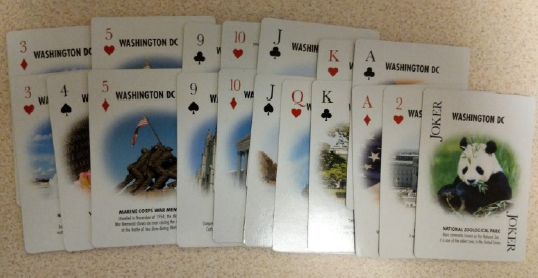
\includegraphics[scale=.5]{h1.png}

\caption{1x15 array representing the counts of each value of card}
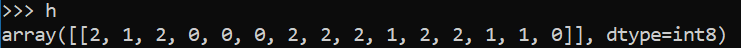
\includegraphics[scale=.5]{h2.png}

\caption{5x15 array with each column being a one-hot encoding of
whether there are 0, 1, 2, 3, or 4 of a card}
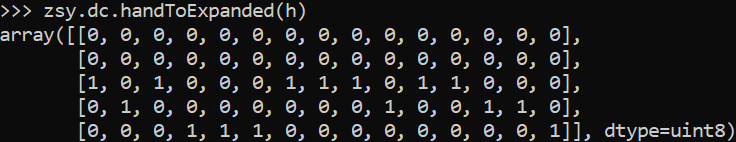
\includegraphics[scale=.5]{h3.png}
\end{center}
\end{figure}

\subsection{Replay Buffer}

In the previous project, I made several models with different hyperparameters and had them running against themselves: they would train for some number of epochs on 100,000 games of data, then dump that data and simulate another 100,000 games against themselves, and repeat. After each simulation, they would test themselves against a random and a greedy agent (that I describe in more detail in section 3), and I periodically manually killed off the worst performing models based on those tests.

That was highly inefficient. This time, I have made a replay buffer inspired by Mnih et al. (2013) that is a halfway in between my old method and theirs. It has a maximum storage of a number of games and keeps indices to every thousand games. Only chunks of 1000 games at a time can be added to the buffer, and when it's full it overwrites the oldest chunk. 

As I test out and train different models, I hope to take advantage of a combined buffer for results of games run between different models, as opposed to each model having its own buffer. While this does introduce more off-policy learning, it will be more data efficient and provide another method for exploration. Algorithm 1 describes my initially intended approach.

\begin{algorithm}[tb]
   \caption{Outline of ideal algorithm}
\begin{algorithmic}
   \STATE Init buffer with 1,000,000 random games
   \STATE Init \textit{M} models
   \REPEAT
   \FOR {m in \textit{M}}
   \STATE Train model m for 1 epoch on buffer
   \ENDFOR
   \FOR {i in range(100,000)}
   \STATE Pick 2 models randomly, weighted by their winrates
   \STATE Simulate a game between those models
   \ENDFOR
   \STATE Add new games to buffer
   \STATE Update model winrates
   \STATE If a model's winrate drops below some threshold, discard model
   \UNTIL{1 model remains}
\end{algorithmic}
\end{algorithm}

\section{First Experiment}

I created 2 agents: a dense network and a CNN. The dense net has 3 layers of size 300, 40, and 1 with ReLu activations for all but the last layer, which has a sigmoid (as the reward is 1 for winning and 0 for losing). The CNN has 2 convolutional layers, first with 32 3x3 filters, the second with 64 3x3 filters, and then dense layers of size 100 and 1; the paddings are valid and all activations but the output layer are ReLu.

As before, state-action pairs are represented by 4 "hands" of cards: the summed agent history, summed opponent history, current agent's cards minus the move, and the move, expanded into one-hot representations and concatenated into a 5x60 array. Unlike Mnih et al. (2013), I decided to use feed each state-action pair into the network to get a Q value. This is because, unlike with the Atari games, the action space is enormous, variable, and discrete. With the different patterns available to play, there a total of 9075 possible actions in the game, with typically 5-30 of them being available on any particular turn. 

As games are episodic with bounded rewards, I decided to use Monte Carlo gains as the targets for the Q network. That is to say, each state-action pair is assigned a value of 1 if it resulted in a victory for the agent and a 0 if it did not.

I initially filled the buffer with 1 million games played by an agent that chooses its moves uniformly at random from its available moves on any particular turn. On average, these games lasted 38 turns, creating ~38 million state-action pairs. 

The agents were each trained for 1 epoch on the data: taking 4096 random samples (without replacement) for each mini-batch and using TensorFlow's implementation of the Adam Optimizer. After training for 1 epoch, I tested both agents against the random agent, a greedy agent (which tries to get rid of as many cards as quickly as possible), and the agent from the previous project. They played 5000 games against each agent, and the results are shown in table 1 with a $2\sigma$ confidence interval on their true winrates. 

However, after each agent trained for a second epoch, the winrates went down across the board.

\begin{table}[t]
\caption{Winrates after 1 epoch}
\label{sample-table}
\vskip 0.15in
\begin{center}
\begin{small}
\begin{sc}
\begin{tabular}{lcccr}
\toprule
Winrate & Dense & Conv  \\
\midrule
vs Random&  62.6 $\pm$ 1.37 & 96.0 $\pm$ 0.56\\
vs Greedy& 41.3 $\pm$ 1.39 & 69.2 $\pm$ 1.31& \\
vs Old DQA& 9.36 $\pm$ 0.82& 35.78 $\pm$ 1.36 \\
\bottomrule
\end{tabular}
\end{sc}
\end{small}
\end{center}
\vskip -0.1in
\end{table}

\begin{table}[t]
\caption{Winrates after 2 epochs}
\label{sample-table}
\vskip 0.15in
\begin{center}
\begin{small}
\begin{sc}
\begin{tabular}{lcccr}
\toprule
Winrate & Dense & Conv  \\
\midrule
vs Random&  48.3 $\pm$ 1.41 & 92.9 $\pm$ 0.72\\
vs Greedy& 35.9 $\pm$ 1.36 & 61.10 $\pm$ 1.38 \\
vs Old DQA& 6.42 $\pm$  0.69 & 25.30 $\pm$ 1.23 \\
\bottomrule
\end{tabular}
\end{sc}
\end{small}
\end{center}
\vskip -0.1in
\end{table}


\section{Second Experiment}
I re-initialized the models and trained them for 1 epoch over only 250k games. They achieved better results than they did 1 epoch over a million, with the CNN already beating out the old model. 

From this, I drew two key points. First, a CNN is a much better approach than a dense network. I had hypothesized a CNN would be useful for picking up on the patterns in the cards, but I had not expected it to be so effective that, trained for only 1 epoch over only 250,000 games completely off-policy, it would already beat out a dense network that was trained over dozens of epochs over many sets of 100,000 games and that was selected from many over a dozen different dense networks. Second, that the buffer size is an important factor to consider. At least from these initial experiments, it seems like a smaller buffer actually works better.


\begin{table}[t]
\caption{Winrates after training over a 250k subset of the buffer}
\label{sample-table}
\vskip 0.15in
\begin{center}
\begin{small}
\begin{sc}
\begin{tabular}{lcccr}
\toprule
Winrate & Dense & Conv  \\
\midrule
vs Random&  78.40 $\pm$ 1.16 & 97.38 $\pm$ 0.45\\
vs Greedy& 53.96 $\pm$ 1.41 & 76.78 $\pm$ 1.19\\
vs Old DQA& 18.98 $\pm$ 1.11 & 55.44 $\pm$ 1.41 \\
\bottomrule
\end{tabular}
\end{sc}
\end{small}
\end{center}
\vskip -0.1in
\end{table}



\section{Next steps}

I will continue to experiment with the buffer size and implement the method I described in the dataset section. I have yet to fully use the buffer as intended: to gradually fading out old games, so I need to experiment on that. I will try different models, but with a heavier focus on different CNNs and perhaps a recurrent network to better capture the history.

\section{References}
Mnih, V., Kavukcuoglu, K., Silver, D., Graves, A., Antonoglou, I., Wierstra, D., \& Riedmiller, M. (2013). Playing Atari with Deep Reinforcement Learning. 

\end{document}


